\newcommand*\justify{%
  \fontdimen2\font=0.4em% interword space
  \fontdimen3\font=0.2em% interword stretch
  \fontdimen4\font=0.1em% interword shrink
  \fontdimen7\font=0.1em% extra space
  \hyphenchar\font=`\-% allowing hyphenation
}

\section{Appendix 2}
\subsection{Guide to dumping memory from Android emulator}\label{guide}
  This guide is based on the guide provided by Volatility \footnote{\url{https://github.com/volatilityfoundation/volatility/wiki/Android}} 
  with more detail and minor modifications.\\
  
  Get the SDK\\
  \texttt{\justify \justify wget https://dl.google.com/android/adt/adt-bundle-linux-x86\_64-20140702.zip} \\
  Unzip SDK\\
  \texttt{\justify unzip adt-bundle-linux-x86\_64-20140702.zip} \\
  Move to better path\\
  \texttt{\justify mv adt-bundle-linux-x86\_64-20140702.zip ~/android-sdk} \\
  To be able to run 32-bit on 64-bit\\
  \texttt{\justify sudo apt-get install libc6-i386 lib32stdc++6} \\
  Move to better path\\
  \texttt{\justify mv android-ndk-r10c ~/android-ndk} \\
  Install required packages\\
  \texttt{\justify sudo apt-get install openjdk-7-jdk bison g++-multilib git gperf libxml2-utils curl} \\
  Set up cache\\
  \texttt{\justify export USE\_CCACHE=1}
  Set ~/bin in your \$PATH
  \texttt{\justify mkdir ~/bin} \\
  \texttt{\justify PATH=~/bin:\$PATH} \\
  Download the repo tool and make it executable\\
  \texttt{\justify curl https://storage.googleapis.com/git-repo-downloads/repo > ~/bin/repo} \\
  \texttt{\justify chmod a+x ~/bin/repo} \\
  Create repo dir\\
  \texttt{\justify mkdir ~/android-repo \&\& cd ~/android-repo} \\
  Set git git config if you have not done so already\\
  \texttt{\justify git config --global user.email "you@example.com"} \\
  \texttt{\justify git config --global user.name "Your Name"} \\
  Initialize repo\\
  \texttt{\justify repo init -u https://android.googlesource.com/\\platform/manifest} \\
  Sync repo (this will take a long time and take up approximately 31 GB)\\
  \texttt{\justify repo sync} \\
  set up environment\\
  \texttt{\justify . build/envsetup.sh} \\
  Set some variables\\
  \texttt{\justify lunch full-eng} \\
  Update the SDK\\
  \texttt{\justify android update sdk -u} \\
  Before creating the AVD, you need the Image for the target we are using (4.2 API Level 17).\\
  \texttt{\justify android sdk} \\
  Select "ARM EABI v7a System Image" under API 17 and Install\\
  Create avd\\
  \texttt{\justify android avd} \\
  Set AVD name to "myavd", Device to Nexus 7 (2012) and Target to 4.2 (API Level 17). Select "Display skin with hardware controls". 
  Make sure to set the SD-card size to larger than the amount of RAM, beacuse we are saving RAM to SD-card. 
  We set 2 GB. Select Use host GPU.\\
  
  Download the Kernel source\\
  \texttt{\justify git clone https://android.googlesource.com/kernel/goldfish.git ~/android-source} \\
  \texttt{\justify cd ~/android-source/} \\
  Change branch to android-goldfish-2.6.29\\
  \texttt{\justify git checkout android-goldfish-2.6.29} \\
  Before Compiling the kernel we need to set som variables\\
  \texttt{\justify export ARCH=arm} \\
  \texttt{\justify eexport SUBARCH=arm} \\
  \texttt{\justify export CROSS\_COMPILE=arm-eabi-} \\
  Create the config file\\
  \texttt{\justify make goldfish\_armv7\_defconfig} \\
  Open the config file, and make sure the following is set:\\
  \texttt{\justify CONFIG\_MODULES=y\\ CONFIG\_MODULES\_UNLOAD=y\\ CONFIG\_MODULES\_FORCE\_UNLOAD=y\\ } \\
  Build the kernel. (when asked questions, just press enter for the default)\\
  \texttt{\justify make} \\
  You can now start the emulator\\
  \texttt{\justify emulator -avd myavd -kernel ~/android-source/arch/arm/boot/zImage -show-kernel -verbose} \\
  Download LiME\\
  \texttt{\justify git clone https://github.com/504ensicsLabs/LiME.git ~/LiME} \\
  \texttt{\justify cd ~/LiME/src} \\
  Edit the Makefile to correspond to this diff:\\
  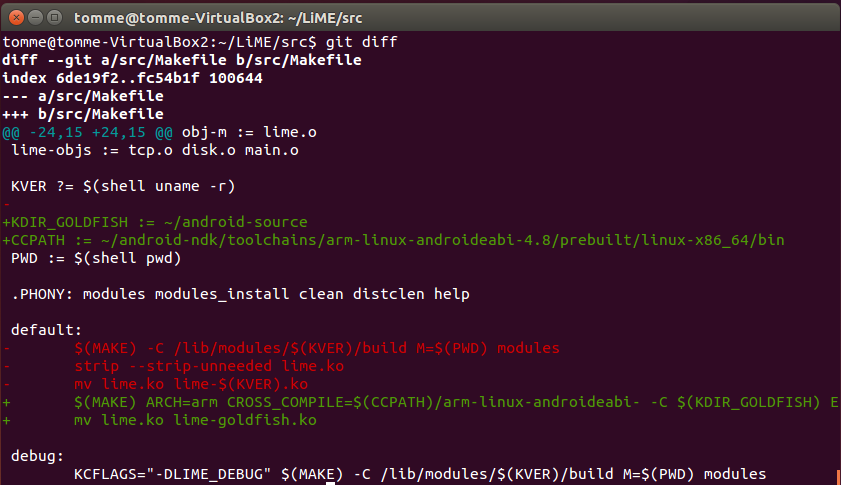
\includegraphics[scale=0.5]{diff.png} \\
  Make the kernel module\\
  \texttt{\justify make} \\
  Push the kernel module to the emulator\\
  \texttt{\justify ~/android-sdk/sdk/platform-tools/adb push ~/LiME/lime-goldfish.ko /sdcard/lime.ko} \\
  Start up a shell on the emulator\\
  \texttt{\justify ~/android-sdk/sdk/platform-tools/adb shell} \\
  In the shell type:\\
  \texttt{\justify insmod /sdcard/lime.ko "path=/sdcard/lime.dump format=lime"} \\
  You now have your memory dump in /sdcard/lime.dump\\
  Transfer it yo your PC and you you can analyse it with volatility or other tools.
  
  
